The Described Constellations are weighted and averaged in the table below. The detailed explanation of the parameters can be found in \ref{PerfAnal}:

\begin{table}[H]
\centering
\begin{tabular}{ | l | c | c | c | c | c | c | c | c | }
\hline
	 &  & \multicolumn{7}{c|} {Candidates}  \\ \hline
	Criteria & W & 1 & 2 & 3 & 4 & 5 & 6 & 7 \\ \hline
	Price & 15 & 1 & 2.35 & 5 & 4.94 & 3.21 & 3.92 & 4.67 \\ \hline
	\% Coverage & 4 & 5 & 4.77 & 2.94 & 2.14 & 4.43 & 1 & 3.86 \\ \hline
	Max Gap Time & 3 & 3.12 & 3.62 & 1 & 2.88 & 3.51 & 5 & 4.75 \\ \hline
	\%Quality time & 5 & 4.91 & 4.49 & 4.05 & 1 & 3.19 & 5 & 4.98 \\ \hline
	Average Pass Time & 5 & 1.21 & 1.14 & 1.14 & 1 & 1.90 & 5 & 4.72 \\ \hline
	Num Gaps & 2 & 4.73 & 4.44 & 4.23 & 1 & 3.03 & 4.99 & 5 \\ \hline
	\% Sats above & 6 & 1 & 1 & 5 & 5 & 1 & 5 & 5 \\ \hline
	SUM (p*g) & 40 & 90.42 & 108.17 & 154.19 & 133.29 & 113.94 & 167.71 & 188.21 \\ \hline
	OWA &  & 0.452 & 0.541 & 0.771 & 0.666 & 0.570 & 0.838 & 0.941 \\ \hline
\end{tabular}
\caption{Constellation Configuration OWA Decision}\label{OWA-Constellation}
\end{table}

With this comparison table, the optimum Constellation is option number 7:\\

\textbf{The Astrea Constellation}

\begin{figure}[H]
\begin{center}
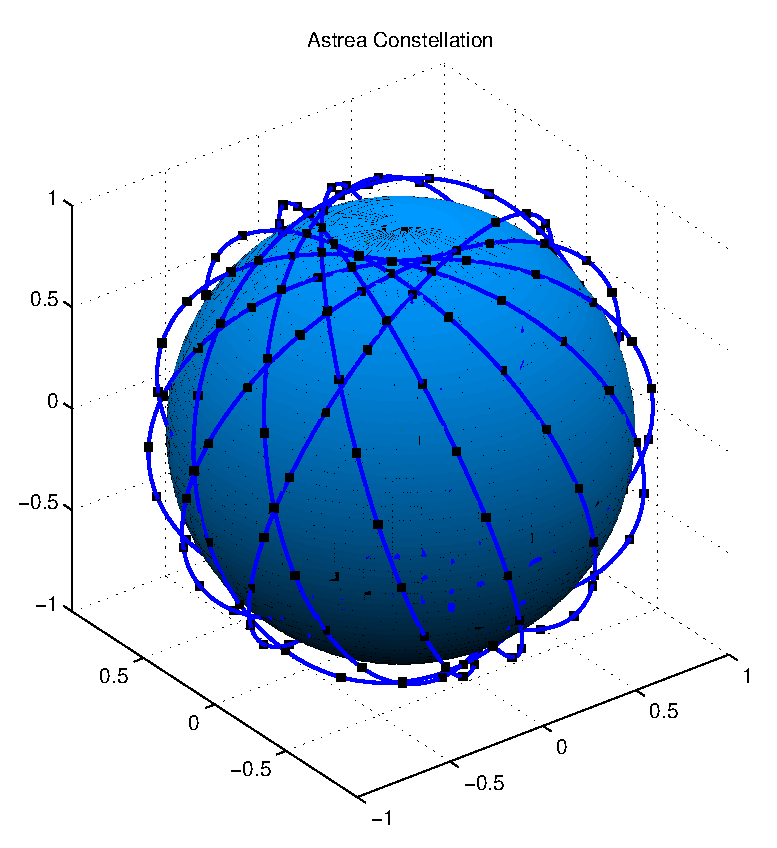
\includegraphics[scale=0.75]{FinalConfig}
\caption{Astrea Constellation Final Configuration.}
\end{center}
\end{figure}
